%%%%%%%%%%%%%%%%%%%%%%%%%%%%%%
\section{Design of estimators}
%%%%%%%%%%%%%%%%%%%%%%%%%%%%%%

%%%%%%%%%%%%%%%%%%%%%%%%%%%%%%%%%%%%%%%%%%%%%%%
\subsection{Maximum Likelihood (ML) estimation}

The maximum likelihood estimator (ML) uses the likelihood as the reward function to be maximized:
\begin{equation}
\sML = \argmax_s p_{{\bf X}|S}({\bf x}|s)
     = \argmax_s \ln(p_{{\bf X}|S}({\bf x}|s))
\label{ec:est_ML}
\end{equation}

The ML estimator selects the value of the parameter $s$ that maximizes the likelihood of observing ${\bf x}$ when $S=s$. Loosely speaking, observing ${\bf x}$ when $S=\sML$ is less unexpected than if $S$ takes any other value. Note that $p_{{\bf X}|S}({\bf x}|s)$, which is a density function over random variable ${\bf X}$, is not maximized with respect to ${\bf x}$, but $s$. 
% Note that in the estimator definition alternatively includes  the use of the logarithm function (or some other with similar properties) and its use does not affect in any case the value resulting from maximization.

%%%%%%%%%%%%%%%
\begin{example}[ML Estimation]
\label{ex:est_ML_varaleat}

We want to estimate the value of a random variable $S$ from an observation $X$ statistically related to it. For the design of the estimator, only the likelihood of $S$ is known, which is given by
\begin{equation}
p_{X|S}(x|s) = \frac{2 x}{(1 - s)^2},\;\; 0 \le x \le 1-s,\;\; 0 \le s \le 1
\end{equation}
Given the available statistical information, it is decided to construct the ML estimator of $S$. The likelihood function represents the probability density of the random variable $X$, normalized to have unit area, as represented in Figure \ref{fig:est_ML_caso1}(a). However, to carry out the maximization, representing this likelihood as a function\footnote{Note that the integral with respect to $s$ of $p_{X|S}(x|s)$ will not generally be the unit, since this function does not constitute a probability density of $S$.} of $s$ (Fig.\ref{fig:est_ML_caso1}(b)) is more useful, as it shows that the estimator is
$$\hat s_{\text{ML}} = 1 - x$$
or, alternatively, if we consider the application of the estimation function on the random variable $X$ instead of on a specific value of it,
$$\hat S_{\text{ML}} = 1 - X$$

%%%%%%%%%%%%%%
\begin{figure}[t]
  \begin{center}
  \begin{tabular}{cc}
    %\epsfig{file=Figures/px_s_funcionx, width=6cm} 
    \includegraphics[width=6cm]{Figures//px_s_funcionx.png} &
   % \epsfig{file=Figures/px_s_funcions, width=6cm} \\ 
   
   \includegraphics[width=6cm]{Figures//px_s_funcions.png}\\
    (a) & (b)
  \end{tabular}
    \caption{Representation of the likelihood distribution of the example \ref{ex:est_ML_varaleat} as a function of $x$ and $s$.}
    \label{fig:est_ML_caso1}
  \end{center}
\end{figure}
%%%%%%%%%%%%

\end{example}
%%%%%%%%%%%%%

{Note that the second equality in \eqref{ec:est_ML} states that the maximization of the likelihood is equivalent to the maximization of its logarithm (the \textbf{log-likelihood} function). Since the logarithm function is strictly increasing, $p_{{\bf X}|S}({\bf x}|s_1) > p_{{\bf X}|S}({\bf x}|s_2)$ implies $\ln(p_{{\bf X}|S}({\bf x}|s_1)) > \ln(p_{{\bf X}|S}({\bf x}|s_2))$) and, thus, the logarithm does not alter the outcome of the maximization}. The logarithm is used by practical reasons when the likelihood is a product of several factors or an exponential function, as it will transform products into sums and an exponential into the exponents. In this way, the maximization process can be simplified considerably.

{Note that the maximum likelihood does not need any probability model about the target variable, $S$, which is treated as a deterministic parameter. This is useful in situations where only the likelihood function is known}.


%%%%%%%%%%%%%%%%%%%%%%%%%%%%%%%%%%%%%%%%%%%%%%%%%%
\subsection{Maximum a posteriori (MAP) estimation}

We define the maximum a posteriori (MAP) estimator as the mode of the posterior distribution, that is
\begin{equation}
\hat s_{\text{MAP}} = \argmax_{s} p_{{S|\bf X}}(s|{\bf x})
                    = \argmax_{s} \ln(p_{{S|\bf X}}(s|{\bf x}))
                   \label{ec:est_MAP}
\end{equation}

{Using the definition of conditional pdf and Bayes' rule, it is easy to see that the MAP estimator can be computed as
\begin{align}
\label{eq:est_smap2}
\hat s_{\text{MAP}} 
	&= \argmax_{s} p_{{S,\bf X}}(s,{\bf x})   \\
\label{eq:est_smap3}
    &= \argmax_{s} \{p_{{\bf X}|S}({\bf x}|s) p_S(s)\}
\end{align}}

{Eq. \eqref{eq:est_smap3} demonstrates that the MAP estimator seeks to maximize the likelihood function, modulated by the prior distribution. This integration of the prior distribution allows the MAP estimator to incorporate existing knowledge or assumptions about the target $S$ before observing the data, ${\bf x}$. When the prior distribution, is uniform across the entire range of possible values of $S$, the distinction between the MAP and ML estimators vanishes, as the MAP estimator effectively reduces to the ML estimator.}

{However, when the prior distribution is not uniform, the MAP estimator is biased towards values of the target variable with higher prior probabilities. This shift illustrates the MAP estimator's sensitivity to prior knowledge.}

{Beyond their mathematical formulations, the MAP and ML estimators embody fundamentally different inference philosophies. The ML estimator optimizes the likelihood function, which models the probability of the observed data under various values of the target, treating $s$ as a fixed but unknown parameter. This approach aligns with the \textbf{frequentist paradigm}, which interprets probability as the long-run frequency of events and does not incorporate prior information about $S$.}

{Conversely, the MAP estimator embraces a \textbf{Bayesian framework}, treating the target as a random variable. This perspective allows the incorporation of prior knowledge or beliefs about $S$ through the prior distribution, $p_S(s)$, and the posterior distribution, $p_{{S|\bf X}}(s|{\bf x})$, updates this knowledge based on new evidence from the data. The Bayesian approach, therefore, provides a probabilistic framework for updating beliefs about uncertain parameters in light of new data.}

%%%%%%%%%%%%%%%
\begin{example}[Estimation MAP]
Considering that  
\begin{equation}
p_{S|X}(s|x) = \frac{1}{x^2} s \exp\left(-\frac{s}{x}\right), \qquad  x\ge 0,\quad s \ge 0
\end{equation}
the MAP estimator can be computed by maximizing
\begin{equation}
\ln(p_{S|X}(s|x)) = -2\ln(x) + \ln(s)-\frac{s}{x}, \qquad  x\ge 0,\quad s \ge 0,
\end{equation}
Since $\ln(p_{S|X}(s|x))$ tends to $-\infty$ around $s=0 $ and $s=\infty$, its maximum must be at some intermediate point with zero derivative. Deriving respect to $s$ results in
\begin{equation}
\left.\frac{\partial}{\partial s} \ln p_{S|X}(s|x)\right|_{s=\sMAP} 
	= \frac{1}{\sMAP} - \frac{1}{x} 
	= 0, \qquad  x\ge 0, \quad s \ge 0
\end{equation}
Thus,
\begin{equation}
\sMAP = x
\end{equation}
\end{example}   %\vspace{0.4cm}
%%%%%%%%%%%%%

%%%%%%%%%%%%%%%%%%%%%%%%%%%%%%%%%%%%
\subsection{Minimum risk estimators}

When a cost function is used to evaluate the quality of an estimation for a given estimation problem, one may wonder if we can find a mathematical expression for the estimator minimizing the mean value of the cost, that is, the risk.

{Taking back the formula of the risk, and applying the total expectation theorem, we find
\begin{align}
\label{ec:coste_medio}
R_f = \EE\{c(S,\hat S)\} 
  & = \int_{\bf x} \EE\{c(S,\hat s)|{\bf X} = {\bf x} \} 
               p_{\bf X}(\bf x) d{\bf x}
\end{align}
where $\hat s= f({\bf x})$. That is, the risk is the integral of the conditional risk, and, thus, the estimator minimizing the risk will be such that it minimizes the conditional risk for each observation ${\bf x}$,}
\begin{equation}
\label{ec:est_bayesiano}
{\hat s}^* = \argmin_{\hat s}\;\EE\{c(S,\hat s)|{\bf X} = {\bf x} \}
\end{equation}
We will refer to this estimator as the \textbf{Bayesian estimator} associated with cost function $c()$. 


%%%%%%%%%%%%%%%
\begin{example}[Calculation of a minimum mean square error estimator]
\label{CalculoECM2}
Following the example \ref{CalculoECM}, we can calculate the posterior distribution of $S$ through
\begin{equation}
p_{S|X}(s|x) = \frac{p_{S,X}(s,x)}{p_X(x)}. 
\end{equation}
Knowing that
\begin{equation}
p_{X}(x) = \int_0^1 p_{S,X}(s,x) ds = \int_0^x \frac{1}{x} ds = 1,   \qquad 0\le x\le 1
\end{equation}
we obtain
\begin{equation}
p_{S|X}(s|x) = \left[
\begin{array}{ll}
\frac{1}{x}, & \qquad 0<s<x<1 \\
0,           & \qquad \text{otherwise}
\end{array}
\right.
\end{equation}
The conditional risk will be given by
\begin{align}
\mathbb{E}\{c(S,\hat s)|X=x\} 
   &= \mathbb{E}\{(S-\hat s)^2|X=x\} \nonumber\\
   &= \int_0^1 (s-\hat{s})^2 p_{S|X}(s|x) ds   \nonumber\\
   &= \frac{1}{x} \int_0^x (s-\hat{s})^2 ds  
    = \frac{1}{x} \left(\frac{(x-\hat{s})^3}{3} + \frac{\hat{s}^3}{3} \right)    \nonumber\\
   &= \frac{1}{3}x^2 - \hat{s} x + \hat{s}^2. 
\label{Est:ECMsx}
\end{align}

As a function of $\hat{s}$, conditional risk is a second-degree polynomial, whose minimum can be calculated through differentiation. Since
\begin{align}
\frac{d}{d\hat{s}} \mathbb{E}\{c(S,\hat s)|X=x\} 
   &= - x + 2 \hat{s} ,
\end{align}
the Bayesian estimator associated with the quadratic error is
\begin{equation}
\label{eq:sopt_halfx}
\hat{s}^* = \frac{1}{2}x,
\end{equation}
which matches the estimator $\hat{S}_1$ from the example \ref{CalculoECM}. Therefore, $\hat{S}_1$ is the best possible estimator from the point of view of the mean square error.
\end{example}\vspace{0.4cm}
%%%%%%%%%%%%%

Based on \eqref{ec:est_bayesiano} we can conclude that, regardless of the cost to be minimized, the knowledge of the posterior distribution of $S$ given ${\bf X}$, $p_{S|{\bf X}}(s|{\bf x})$, is sufficient to design the Bayesian estimator for a given cost. As mentioned above, this distribution is often calculated from the likelihood of $S$ and its a priori distribution using the Bayes Theorem, which is in fact the origin of the denomination of these estimators.

\newpage

%%%%%%%%%%%%%%%%%%%%%%%%%%%%%%%%%%%%%%%%%%%%%%%%%
\section{Common Bayesian estimators}
%%%%%%%%%%%%%%%%%%%%%%%%%%%%%%%%%%%%%%%%%%%%%%%%%

This section presents some of the most commonly used Bayesian estimators. For their calculation, we will proceed to minimize the mean cost given $\bf X$ (posterior mean cost) for different cost functions.


%%%%%%%%%%%%%%%%%%%%%%%%%%%%%%%%%%%%%%%%%%%%%%%%%%%%%%%
\subsection{Minimum Mean Squared Error estimator (MSE)}

The minimum mean squared error (MSE) estimator is the Bayesian estimator associated with the cost function $c(e) = e^2 = (s-\hat s)^2$, and therefore is given by 
\begin{align}
\label{ec:coste_medio_cuadratico}
\sMSE 
  & = \argmin_{\hat s} \; \EE\{c(S,\hat s)|{\bf X} = {\bf x} \}   \nonumber\\
  & = \argmin_{\hat s} \; \EE\{(S-\hat s)^2|{\bf X} = {\bf x} \}
\end{align}

Figure \ref{fig:estimador_cuadratico} illustrates the minimum MSE estimation problem. The risk can be obtained by integrating (with respect to $s$) the product of the square error and the posterior pdf of $S$. The argument for minimization is $\hat s$, which allows shifting the graph corresponding to the cost function (represented with discontinuous stroke) so that the result of that integral is minimal.

%%%%%%%%%%%%%%
\begin{figure}[th]
  \begin{center}
    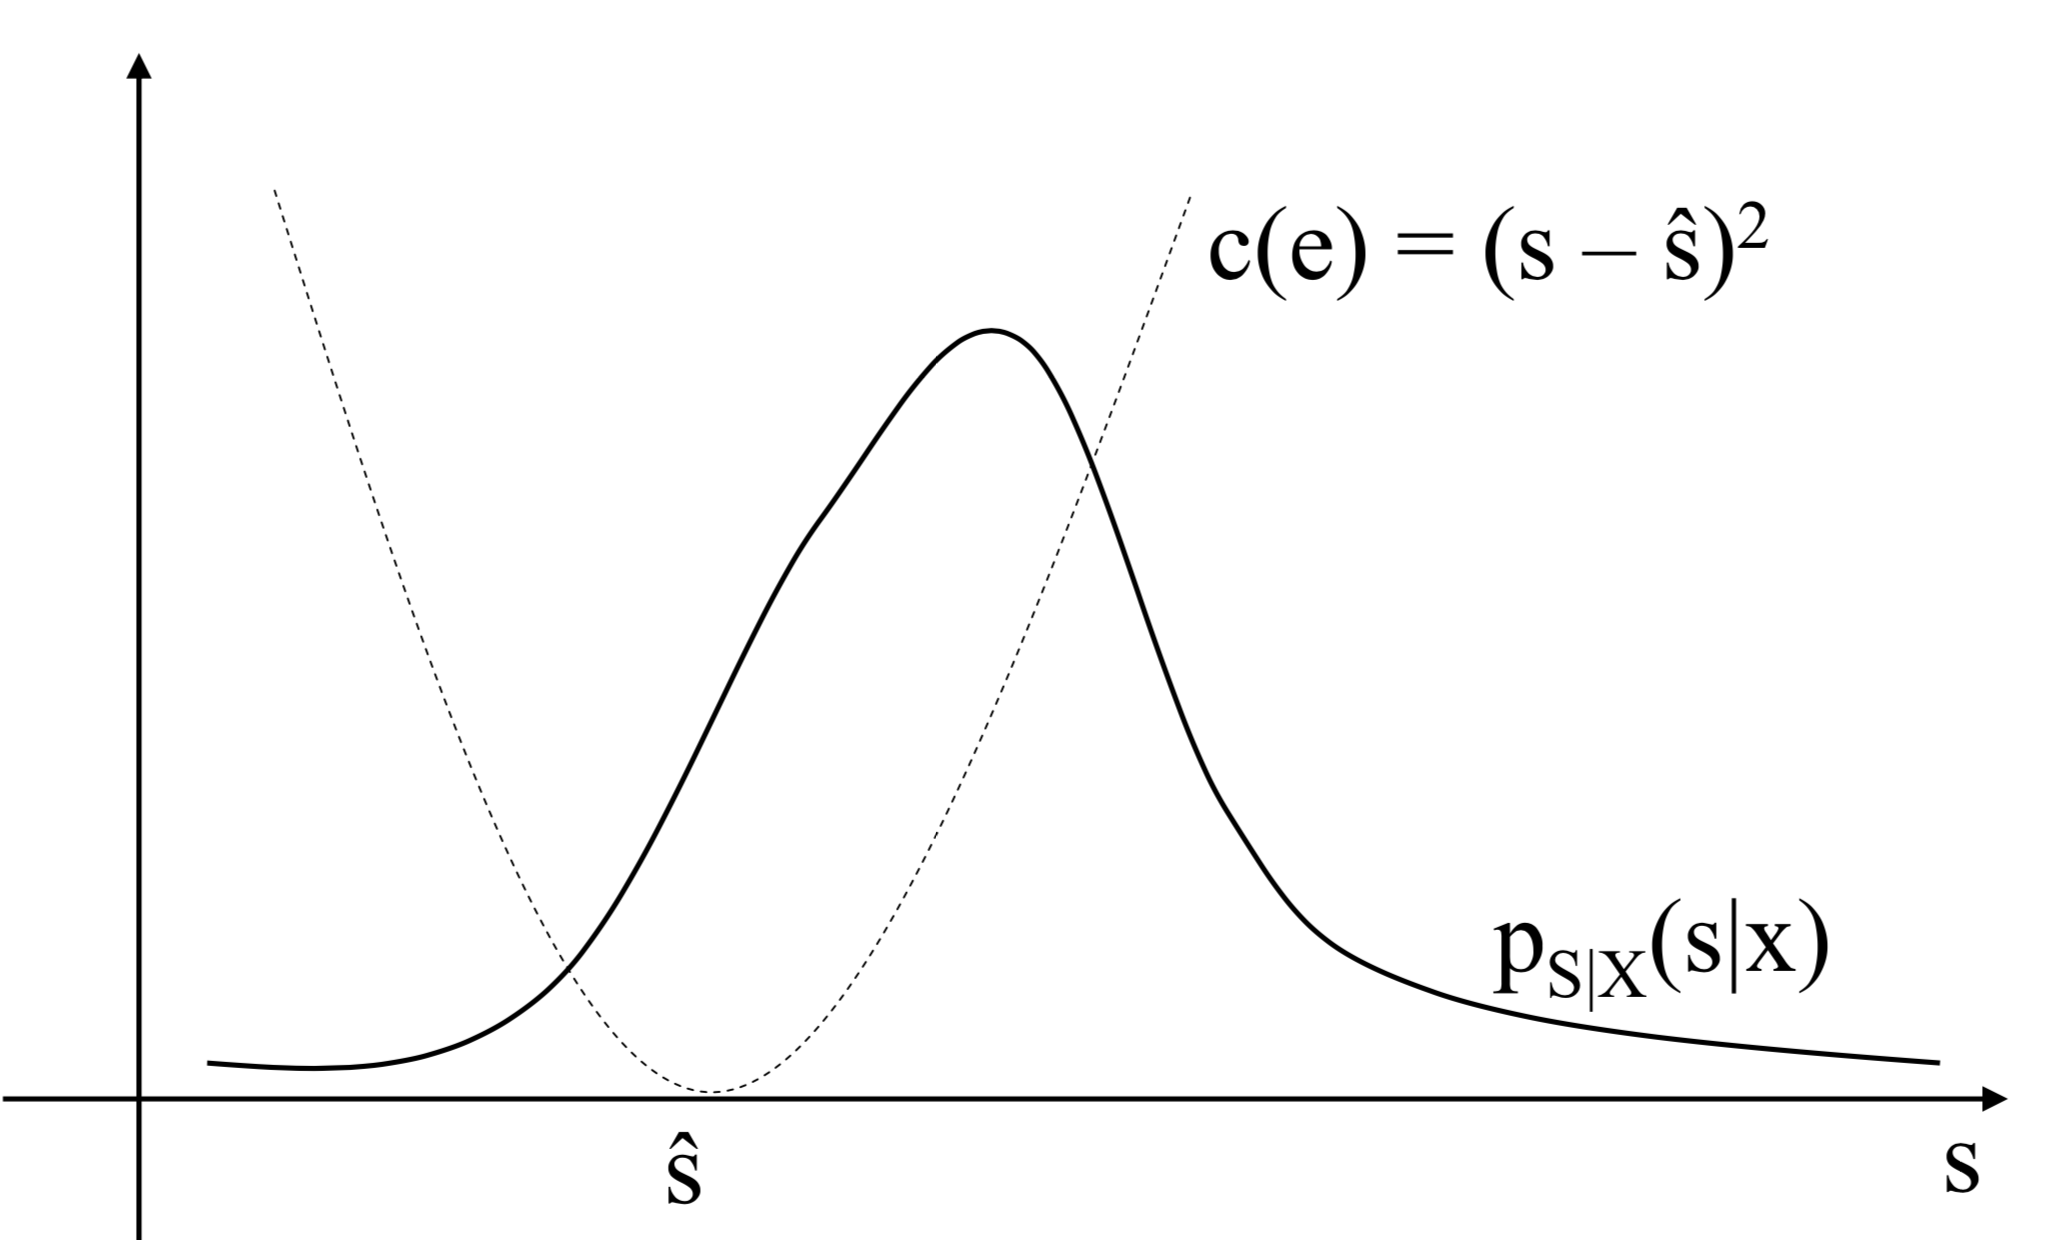
\includegraphics[width=7cm]{Figures//estimador_cuadratico.png}
    \caption{Graphical representation of the process of calculating the posterior mean for a generic value $\hat{s}$.}
    \label{fig:estimador_cuadratico}
  \end{center}
\end{figure}
%%%%%%%%%%%%

{For the square error, the conditional risk in \eqref{ec:coste_medio_cuadratico} becomes
\begin{align}
\label{ec:gen_mse2}
\EE\{(S-\hat s)^2|{\bf X} = {\bf x} \}
    = \EE\{S^2|{\bf X} = {\bf x} \}
    - 2\EE\{S|{\bf X} = {\bf x} \} \hat s
    + \hat s^2
\end{align}
This is a second-degree polynomial that can be minimized by differentiation to get}
%The value of $\hat s_{\text{MSE}}$ can be analytically obtained by taking the derivative of the posterior mean cost and equaling the result to 0. The calculation of the derivative does not pose any difficulty since the derivative and the integral can be commuted (it is integrated with respect to $s$ and is derived with respect to $\hat s$):
%\begin{equation}
%\label{ec:estimador_MSE}
%\left.\frac{d \EE\{(S-\hat s)^2| {\bf X}={\bf x}\}}{d \hat s}\right|_{\hat s = \sMSE} 
% = -2 \int_s (s - \hat s_{\text{MSE}}) p_{S|{\bf X}}(s|{\bf x}) ds = 0
%\end{equation}
% Bearing in mind that the integral in \eqref{ec:estimador_MSE} should be cancelled, and using the fact that $\int p_{S|{\bf X}}(s|{\bf x}) ds = 1$, it is easy to demonstrate that the minimum mean squared error estimator of $S$ is given by
\begin{framed}
\begin{equation}
\label{ec:estimador_MSE_final}
\sMSE = \EE\{S|{\bf X} ={\bf x}\} = \int s\;p_{S|{\bf X}}(s|x) ds
\end{equation}
\end{framed}

In other words, the minimum MSE estimator of $S$ is the posterior mean of $S$ given $\bf X$.

%%%%%%%%%%%%%%%%
%\begin{exercise}
%Check that the expression \eqref{ec:estimador_MSE_final} actually constitutes a minimum of the given average cost {\bf X}, by calculating the second derivative of $\mathbb{E}\c(S,\hat s)|{bf X} = {\bf x}$.
%\end{exercise}
%%%%%%%%%%%%%%


%%%%%%%%%%%%%%%
\begin{example}[Straightforward calculation of the MSE estimator]
According to \eqref{ec:estimador_MSE_final}, minimum mean squared error estimator obtained in \ref{CalculoECM} can alternatively be derived as follows

\begin{align}
\label{ec:estimador_MSE_final2}
\hat s_{\text{MSE}} = \int_0^1 s p_{S|X}(s|x) ds   
   = \int_0^x \frac{s}{x} ds 
   = \frac{1}{2} x
\end{align}
which is consistent with \eqref{eq:sopt_halfx}.
\end{example}\vspace{0.4cm}
%%%%%%%%%%%%%



%%%%%%%%%%%%%%%%%%%%%%%%%%%%%%%%%%%%%%%%%%%%%%%%%%%%%
\subsection{Minimum Mean Absolute Deviation Estimator (MAD)}

In the same way, as we have proceeded in the case of the estimator $\hat s_\text{MSE}$, we can calculate the estimator associated with the absolute deviation of the estimation error, $c(e) = |e| = |s - \hat s|$. This estimator, which we will refer to as the Mean Absolute Deviation (MAD), is characterized by

\begin{align}
\label{ec:coste_MAD}
\sMAD & = \argmin_{\hat s}\; \EE\{|S - \hat s|~|{\bf X} = {\bf x} \} = \\
	  & = \argmin_{\hat s}   \int_s |s - \hat s|\;p_{S|{\bf X}}(s|{\bf x}) ds
\end{align}

Again, it is simple to illustrate the process of calculating the posterior mean cost by overlapping on the same axes the cost expressed as a function of $s$ and the posterior distribution of the variable to be estimated (see Fig. \ref{fig:estimador_absoluto}). This representation also suggests the convenience of splitting the integral into two parts corresponding to the two slopes of the cost function:
\begin{align}
\EE\{|S - \hat s|~|{\bf X} = {\bf x} \} 
	=& \int_{-\infty}^{\hat s} (\hat s - s) \;p_{S|{\bf X}}(s|{\bf x}) ds
		+ \int_{\hat s}^\infty (s - \hat s) \;p_{S|{\bf X}}(s|{\bf x}) ds \\
	=& \hat s \left[  \int_{-\infty}^{\hat s} p_{S|{\bf X}}(s|{\bf x}) ds 
				    - \int_{\hat s}^{\infty}  p_{S|{\bf X}}(s|{\bf x}) ds \right] \\
	 &  + \int_{\hat s}^{\infty}  s \; p_{S|{\bf X}}(s|{\bf x}) ds 
		- \int_{-\infty}^{\hat s} s \; p_{S|{\bf X}}(s|{\bf x}) ds
\end{align}

%%%%%%%%%%%%%%
\begin{figure}[t]
  \begin{center}
  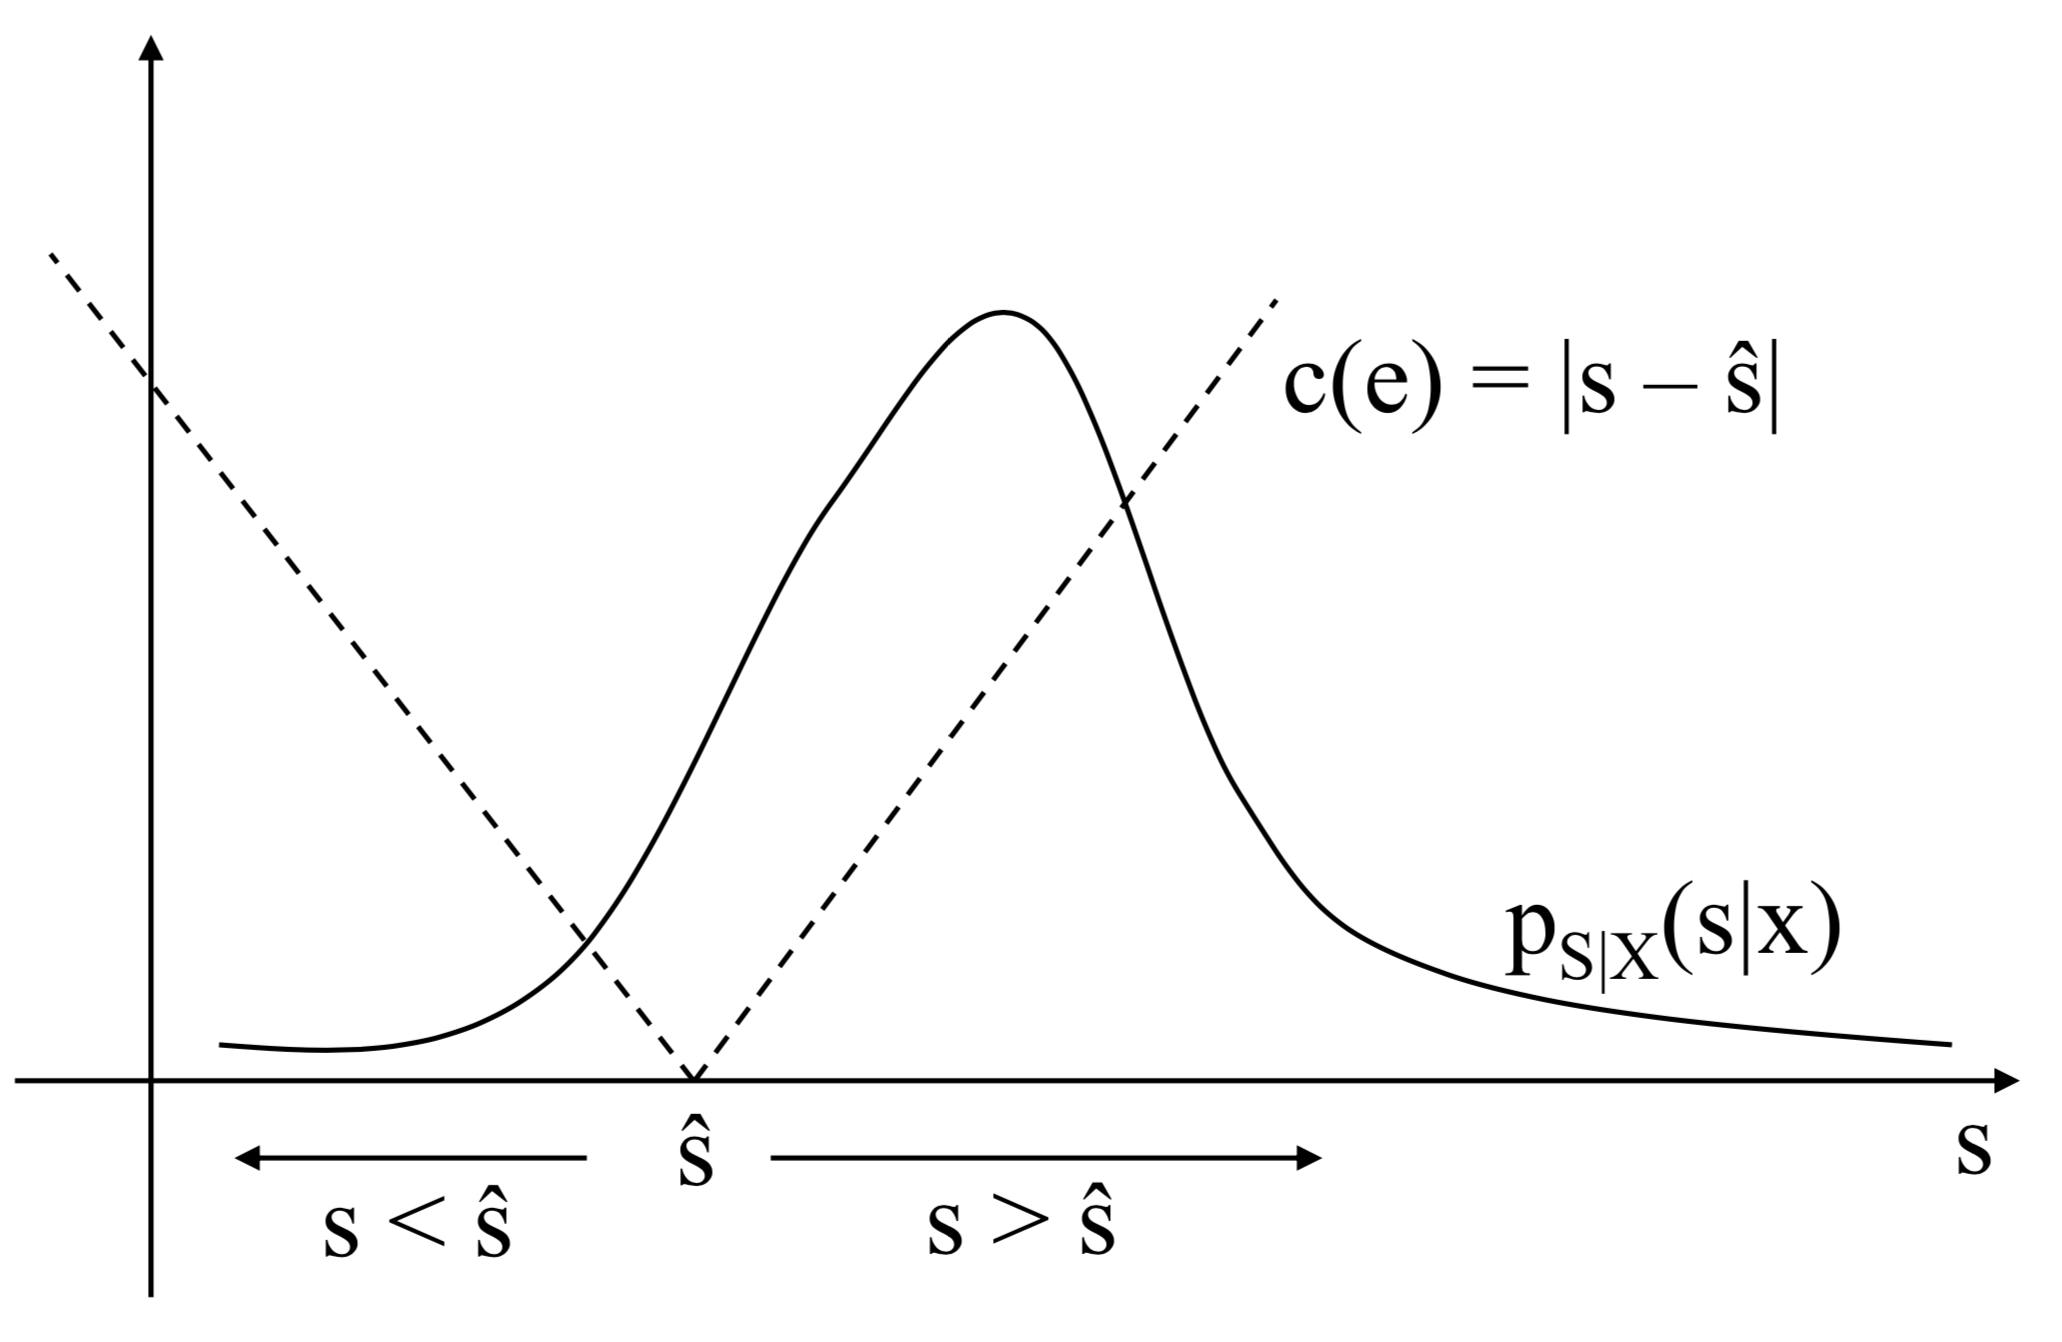
\includegraphics[width=7cm]{Figures//estimador_absoluto.png}
    \caption{Calculation of the posterior mean absolute error for a generic value $\hat s$.}
    \label{fig:estimador_absoluto}
  \end{center}
\end{figure}
%%%%%%%%%%%%

The fundamental theorem of calculus\footnote{$\frac{d}{d x} \int_{t_0}^x g(t) dt = g(x)$.} allows us to obtain the derivative of the conditional risk as
\begin{equation}
\frac{d \mathbb{E}\{|S - \hat s|~|{\bf X} = {\bf x} \}}{d \hat s} 
    = 2 F_{S|{\bf X}}(\hat s|{\bf x}) - 1
\end{equation}
where $F_{S|{\bf X}}(s|{\bf x})$ is the posterior distribution function of $S$ given ${\bf X}$. Since this derivative must vanish at the \textcolor{magenta}{minimum}, we get $F_{S|{\bf X}}(\hat s_{\text{MAD}}|{\bf x}) = 1/2$. In other words, the \textcolor{magenta}{minimum MAD} estimator is given by the median of $p_{S|{\bf X}}(s|{\bf x})$:

\begin{framed}
\begin{equation}
\label{ec:estimador_MAD_final}
\hat s_{\text{MAD}} = \text{median}\{S|{\bf X} ={\bf x}\}
\end{equation}
\end{framed}

Remember that the median of a distribution is the point that separates that distribution into two regions that have the same probability, so the minimum \textcolor{magenta}{MAD} estimator \textcolor{magenta}{satisfies}
\textcolor{magenta}{\begin{align}
P\{S > \sMAD |{\bf x}\} = P\{S < \sMAD |{\bf x}\}
\end{align}}

In practice, this can be computed as the solution of
\begin{align}
\int_{-\infty}^{\sMAD} p_{S|{\bf X}}(s|{\bf x}) ds = \frac12
\end{align}


\begin{example}[Design of a Minimum Mean Absolute Deviation Estimator]

In the scenario of the example \ref{CalculoECM}, the posterior distribution of $S$ given $X$ is uniform between 0 and $x$, the median of which is $x/2$. Thus,
\begin{align}
\label{ec:estimador_MSE_finalej}
\sMAD = \frac{1}{2} x 
\end{align}

Note that, in this case, the MAD estimator matches the MSE obtained at \eqref{eq:sopt_halfx}. This is a consequence of the symmetry of the a posterior distribution.
\end{example}



